\section{Problems of Kuberenetes}

\begin{figure}
  \centering
  \includegraphics[width=0.8\columnwidth]{Figs/K8sConventional}
  \caption{Conventional architecture of a Kubernetes cluster.}
  \label{fig:K8sConventional}
\end{figure}

Problems commonly occur when the Kubernetes container management system is used outside of recommended cloud providers(such as GCP or AWS).
Figure~\ref{fig:K8sConventional} shows an exemplified Kubernetes cluster.
A Kubernetes cluster typically consists of a master and nodes. They can be physical servers or VMs.
On the master, daemons that control the Kubernetes cluster are typically deployed. 
These daemons include, apiserver, scheduler, controller-manager and etcd. 
On the nodes, the kubelet daemon will run {\it pods}, depending the PodSpec information obtained from the apiserver on the master.
A {\em pod} is a group of containers that share same net name space and cgroups, 
and is the basic execution unit in a Kubernetes cluster.

When a service is created, the master schedules where to run {\em pods} and kubelets on the nodes launch them accordingly.
At the same time, the master sends out requests to cloud provider API endpoints, asking them to set up external cloud load balancers.
The proxy daemon on the nodes also setup iptables DNAT\cite{MartinA.Brown2017} rules. 
The Internet traffic will then be evenly distributed by the cloud load balancer to nodes, 
after which it will be distributed again by the DNAT rules on the nodes to the designated {\em pods}. 
The returning packets follows the exact same route as the incoming ones.

This architecture has the followings problems: 
1) There must exist cloud load balancers whose APIs are supported by the Kubernetes daemons.
There are numerous load balancers which is not supported by the Kubernetes.
These include the bare metal load balancers for on-premise data centers.
2) Distributing the traffic twice, first on the external load balancers and second on each node, complicates the administration of packet routing. 
Imagine a situation in which the DNAT table on one of the nodes malfunctions.
In such a case, only occasional timeouts would be observed, which would make it very difficult to find out which node was malfunctioning.   

Regarding the first proble, if there is no load balancer that is not supoorted by Kubernetes, users might be able to set up the routing manually depending on the infrastructure.
The traffic would be routed to a node then distributed by the DNAT rules on the node to the designated {\em pods}.
However, this approach significantly degrades the portability of container clusters.

In short, 1) Kubernetes can be used only in limited environments where the external load balancers are supported, and 2) the routes incoming traffic follow are very complex.
In order to address these problems, we propose a containerized software load balancer 
that is deployable in any environment even if there are no external load balancers.

\section{Proposed Architecture}

This chapter discusses the load balancer architecure.
How they are implemented and how redandancy is realized.

The porblems of Kubernetes architecture in Figure~\ref{fig:K8sProposed} have been the followings;
1) There are environments with load balancers whoes APIs are not supported by Kubernetes.
2) Incomming traffic are distributed twice, once at the load balancer and once at the every node.

There are several possible ways to solve these problems.
a) Make Kubernetes support all of exisiting load balancer hardwares that could be used in on-premise data centers.
b) Force users to buy new load balancer that is supported by Kubernetes.
c) Provide software load balancers and make them supported by Kubernetes.
d) Provide software load balancers as a part of container cluters.

The a) is impossible. The b) does not improve usability of container cluster since specific hardwares are always needed.
The c) and d) are viable solutions since they are realized using commodity hardware.

We do not know how many load balancers are needed for a specific web service.
We also do not know how many of the services are deployed in a data center.
Therefore a cluster of load balancers should be elastice, i.e. it should change the capacity on demand.
And we also should be able to deploy many of load balancer cluster on demand.
It would be better if we could share the same server pool with web servers, since capacity planning for hardwares to host load balancer clustes may be difficult.

For such application needs the container cluster seems best suited.
Therefore the author proposes the architecture where a cluster of load balancers are also deployed as a cluster of containers.

\begin{figure}
  \centering
  \includegraphics[width=0.8\columnwidth]{Figs/K8sProposed}
  \caption{Kubernetes cluster with proposed load balancer.}
  \label{fig:K8sProposed}
\end{figure}

Figure~\ref{fig:K8sProposed} shows the proposed laod balancer architecture for Kubernetes,
which has the following characteristics:
1) Each load balancer itself is run as a {\em pod} by Kubernetes. 
2) Balancing tables are dynamically updated based on information about running {\em pods}.
3) There exist multiple load balancers for redundancy.
4) The routes to load balancers in the upstream router are updated dynamically.
The proposed load balancer can resolve the conventional architecture problems, as follows:
Since the load balancer itself is containerized, the load balancer can run in any environment including on-premise data centers, even without external load balancers that is supported by Kubernetes.
Load balancers can share the server pool with web containers.
The incoming traffic is directly distributed to designated {\em pods} by the load balancer. 
It makes the administration, e.g. finding malfunctions, easier.

\section{Portable Load Balancer}

The proposed load balancer uses three components, ipvs, keepalived, and a controller. 
These components are placed in a Docker container image.
The ipvs is a Layer-4 load balancer capability, which is included in the Linux kernel 2.6.0 released in 2003 or later, 
to distribute incoming Transmission Control Protocol(TCP) traffic to 
{\em real servers}\footnote{The term, {\em real servers} refers to worker servers that will respond to incoming traffic, 
in the original literature\cite{Zhang2000}. We will also use this term in the similar way.}\cite{Zhang2000}. 
For example, ipvs distributes incoming Hypertext Transfer Protocol(HTTP) traffic destined for a single destination IP address, 
to multiple HTTP servers(e.g. Apache HTTP or nginx) running on multiple nodes in order to improve the performance of web services.
Keepalived is a management program that performs health checking for {\em real servers}
and manages ipvs balancing rules in the kernel accordingly.
It is often used together with ipvs to facilitate ease of use.
The controller is a daemon that periodically monitors the {\em pod} information on the master, 
and it performs various actions when such information changes.
Kubernetes provides ingress controller framework as the Go Language(Golang) package to implement the controllers. 
We have implemented a controller program that feeds {\em pod} state changes to keepalived 
using this framework. 

\section{Routing and Redundancy}

While containerizing ipvs makes it runnable in any environment, it is essential to discuss how to route the traffic to the ipvs container.
We propose redundant architecture using ECMP for load balancer containers usable especially in on-premise data centers.
We first explain the proposed architecture with ECMP redundancy in \ref{Redundancy with ECMP}, then  present an alternative architecture using VRRP as a comparison in \ref{Redundancy with VRRP}, which we think is not as good as the architecture using ECMP.

\subsection{ECMP}\label{Subsec:Redundancy with ECMP}

\begin{figure}[tb]
  \centering
  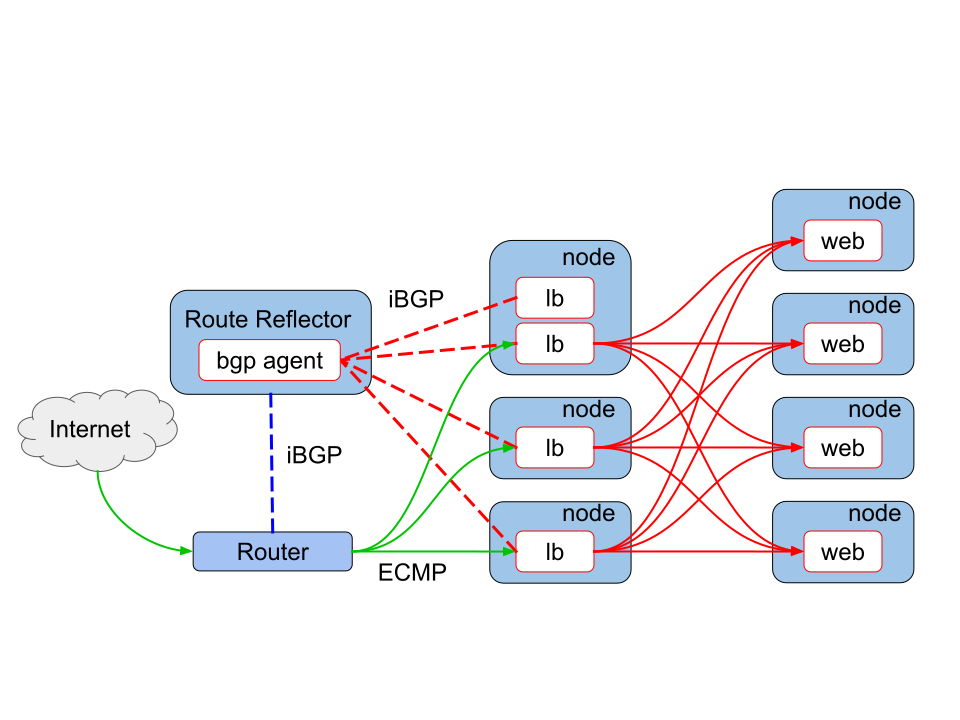
\includegraphics[width=0.8\columnwidth]{Figs/ecmp.png}
\caption{
  The proposed architecture of load balancer redundancy with ECMP. %\\ %\par 
  The traffic from the internet is distributed by the upstream router to multiple of lb pods using hash-based ECMP and then distributed by the lb pods to web pods using Linux kernel's ipvs.
  The ECMP routing table on the upstream router is populated using iBGP.
}
\label{fig:ecmp}
\end{figure}

Fig.~\ref{fig:ecmp} shows our proposed redundancy architecture with ECMP for software load balancer containers.
%
The ECMP is a functionality a router often supports, where the router has multiple next hops with equal cost(priority) to a destination, and generally distribute the traffic depending on the hash of the flow five tuples(source IP, destination IP, source port, destination port, protocol).
The multiple next hops and their cost are often populated using the BGP protocol.
%
The notable benefit of the ECMP setup is the fact that it is scalable.
All the load balancers that claims as the next hop is active, i.e., all of them are utilized to increase the performance level.
Since the traffic from the internet is distributed by the upstream router, the overall throughput is determined by the router after all.
However, in practice, there are a lot of cases where this architecture is beneficial.
For example, if a software load balancer is capable of handling 1 Gbps equivalent of traffic and the upstream router is capable of handling 10 Gbps, it still is worthwhile launching 10 of the software load balancer containers to fill up maximum throughput of the upstream router.

%
We place a node with the knowledge of the overlay network as a route reflector, to deal with the complexity due to the SNAT.
A route reflector is a network component for BGP to reduce the number of peerings by aggregating the routing information\cite{rfc4456}.
In our proposed architecture we use it as a delegater for load balancer containers towards the upstream router.

By using the route reflector, we can have the following benefits.
1) Each node can accommodate multiple load balancer containers. This was not possible when we tried to directly connect load balancers and the router through SNAT.
2) The router does not need to allow peering connections from random IP addresses that may be used by load balancer containers. Now, the router only need to have the reflector information as the BGP peer definition.

Since we use standard Linux boxes for route reflectors, we can configure them as we like;
a) We can make them belong to overlay network so that multiple BGP sessions from a single node can be established.
b) We can use a BGP agent that supports dynamic neighbor (or dynamic peer), where one only needs to define the IP range as a peer group and does away with specifying every possible IP that load balancers may use.

The upstream router does not need to accept BGP sessions from containers with random IP addresses, but only from the router reflector with well known fixed IP address. This may be preferable in terms of security especially when a different organization administers the upstream router.
Although not shown in the Fig.~\ref{fig:ecmp}, we could also place another route reflector for redundancy purpose.

\subsection{VRRP}\label{Subsec:Redundancy with VRRP}

\begin{figure}[tb]
\centering
\includegraphics[width=0.8\columnwidth]{Figs/vrrp.png}
\caption{
  An alternative redundant load balancer architecture using VRRP. \\ %\par 
  The traffic from the internet is forwarded by the upstream router to a active lb node and then distributed by the lb pods to web pods using Linux kernel's ipvs.
  The active lb pod is selected using VRRP protocol.
}
\label{fig:vrrp}
\end{figure}

Fig.~\ref{fig:vrrp} shows an alternative redundancy setup using the VRRP protocol that was first considered by the authors, but did not turn out to be preferable.
In the case of VRRP, the load balancer container needs to run in the node net namespace for the following two reasons.
1) When fail over occurs, the new master sends gratuitous Address Resolution Packets(ARP) packets to update the ARP cache of the upstream router and Forwarding Data Base(FDB) of layer 2 swicthes during the transition.
Such gratuitous ARP packets should consist of the virtual IP address shared by the load balancers and the MAC address of the node where the new master load balancer is running.
Programs that send out gratuitous ARP with node MAC address should be in the node net namespace.
%
2) Furthermore, the active load balancer sends out periodic advertisement using UDP multicast packet to inform existence of itself.
The load balancer in backup state stays calm unless the VRRP advertisement stops for a specified duration of time.
The UDP multicast is often unsupported in overlay network used by container cluster environment, and hence the load balancer needs to be able to use the node net namespace.
%
Running containers in the node net namespace loses the whole point of containerization, i.e., they share the node network without separation.
This requires the users' additional efforts to avoid conflict in VRRP configuration for multiple services.
%

VRRP programs also support unicast advertisement by specifying IP addresses of peer load balancers before it starts.
However, container cluster management system randomly assign IP addresses of containers when it launches them, and it is impossible to know peer IPs in advance. 
Therefore the unicast mode is not feasible in container cluster environment.

The other drawback compared with the ECMP case is that the redundancy of VRRP is provided in Active-Backup manner.
This means that a single software load balancer limits the overall performance of the entire container cluster.
Therefore we believe the ECMP redundancy is better than VRRP in our use cases.


\subsection{Kubernetes}

In the Cloud environment BGP peering services are not offered.
In such cases, a Load balancer should update the routing table of cloud infrastructure.


